%% Machine Learning with Applications — Elsevier
%% English version v2 (simplified prose)
%%
%% Compile:
%%   pdflatex main_en_v2
%%   bibtex   main_en_v2
%%   pdflatex main_en_v2
%%   pdflatex main_en_v2

\documentclass[preprint,12pt,authoryear]{elsarticle}

%% ── Packages ──────────────────────────────────────────────────────────────
\usepackage{amsmath,amssymb,amsfonts}
\usepackage{graphicx}
\usepackage{booktabs}
\usepackage{array}
\usepackage{multirow}
\usepackage[table,xcdraw]{xcolor}
\usepackage{hyperref}
\usepackage{cleveref}
\usepackage{lineno}
\usepackage{microtype}
\usepackage{siunitx}
\usepackage{bm}
\usepackage{caption}
\usepackage{subcaption}
\usepackage{enumitem}
\usepackage{algorithm}
\usepackage{algpseudocode}
\algrenewcommand\algorithmicwhile{\textbf{while}}
\algrenewcommand\algorithmicdo{\textbf{do}}
\algrenewcommand\algorithmicend{\textbf{end}}
\algrenewcommand\algorithmicfor{\textbf{for}}
\algrenewcommand\algorithmicif{\textbf{if}}
\algrenewcommand\algorithmicthen{\textbf{then}}
\algrenewcommand\algorithmicelse{\textbf{else}}
\algrenewcommand\algorithmicreturn{\textbf{return}}
\floatname{algorithm}{Algorithm}
\usepackage[utf8]{inputenc}
\usepackage[T1]{fontenc}
\usepackage[english]{babel}

%% Line numbering (required for review)
\linenumbers

\sisetup{separate-uncertainty=true, group-separator={,}, output-decimal-marker={.}}

\hypersetup{
    colorlinks=true,
    linkcolor=blue!70!black,
    citecolor=blue!60!black,
    urlcolor=blue!60!black
}

%% ── Macros ────────────────────────────────────────────────────────────────
\newcommand{\CR}[1]{CR_{2,\text{#1}}}
\newcommand{\RMSE}{\mathrm{RMSE_{CV}}}       % cross-validation
\newcommand{\Rsq}{R^{2}_{\mathrm{CV}}}
\newcommand{\nd}{N_{\mathrm{d}}}
\newcommand{\np}{n_{\mathrm{p}}}              % number of stories
\newcommand{\etad}{\eta}
\newcommand{\Mf}{M_{\!f}}
\newcommand{\ha}{h_a}
\newcommand{\KM}{\,\si{kN{\cdot}m}}

\journal{Machine Learning with Applications}

\begin{document}

\begin{frontmatter}

\title{Machine Learning-Based Optimization of Rotational Friction Dampers in
       Steel Moment-Resisting Frames under Seismic Excitation}

\author[uaq]{E.~Ponce}
\author[i2m]{H.~Yañez-Godoy\corref{cor1}}
\cortext[cor1]{Corresponding author.}
\ead{humberto.yanez-godoy@u-bordeaux.fr}

\address[uaq]{Universidad Autónoma de Querétaro, Faculty of Engineering,
              Cerro de las Campanas s/n, Querétaro, Mexico}
\address[i2m]{Arts et Metiers Institute of Technology, University of Bordeaux,
              Centre National de la Recherche Scientifique (CNRS),
              Bordeaux INP, I2M, UMR 5295, 33400 Talence, France}

%%─── Abstract ───────────────────────────────────────────────────────────────
\begin{abstract}
This study presents a machine learning (ML) based surrogate model framework for
seismic optimization of rotational friction dampers (RFD) in multi-story
moment-resisting steel frames (MRSF). Using Latin Hypercube Sampling (LHS), we
generated 1,000 structurally diverse shear-type frames (3--20 stories, fundamental
period $T_1 \in [0.3,\,3.0]$\,s, mass 150--350 ton/story), evaluating
approximately 50 RFD configurations and 8 real seismic records, yielding
$\approx$434,000 nonlinear time-history simulations solved via Nonsmooth Dynamics
(NSD). The composite performance index $CR_2$ ---integrating normalized maximum
displacement, absolute maximum acceleration, and maximum base shear relative to the
bare frame--- was synthesized across records in three statistical scenarios: median
(typical), P10 (favorable), and P90 (conservative). Four supervised regression
models were trained with GroupKFold cross-validation to prevent information leakage
across structures. XGBoost achieved the best generalization with $\Rsq$ of 0.92,
0.93, and 0.84 for $\CR{med}$, $\CR{P10}$, and $\CR{P90}$, respectively. Variable
importance analysis reveals that damper density $\etad = \nd/\np$ is the dominant
design variable ($r=-0.73$ with $CR_2$), substantially outperforming absolute device
count ($r=-0.45$). An intra-structure analysis demonstrates that 80\% of maximum
achievable improvement is obtained at coverage $\etad \approx 0.85$ for mid-rise and
high-rise frames (6--20 stories), establishing a practical diminishing returns
threshold that quantitatively extends the energy-based findings of \citet{Jarrahi2020sdee}.
\end{abstract}

\begin{keyword}
Rotational Friction Dampers \sep Machine Learning \sep Seismic Optimization \sep
Nonsmooth Dynamics \sep Steel Frames \sep Surrogate Model \sep Diminishing Returns
\end{keyword}

\end{frontmatter}

%%═══════════════════════════════════════════════════════════════════════════
\section{Introduction}
\label{sec:intro}
%%═══════════════════════════════════════════════════════════════════════════

Rotational friction dampers (RFD) are passive devices that improve the seismic
performance of steel frames by dissipating energy through friction
\citep{pall_friction_1980, pall_response_1982, jaisee_state---art_2021}.
\citet{Mualla2002} proposed and tested this device on a single-story frame under
dynamic loading. The device dissipated up to 89\% of input energy. Under the
El~Centro NS record, an optimized case showed 89\% reduction in lateral
displacement and 41\% reduction in base shear compared to the uncontrolled frame.

Unlike conventional designs that allow energy dissipation through inelastic
deformation of frame members, RFDs transfer a large portion of that dissipation to
a dedicated friction mechanism. This reduces demand on primary structural elements
and produces a more controlled seismic response \citep{de_domenico_editorial_2020}.

Modeling these devices is difficult because dry friction is inherently nonlinear.
Past numerical studies have used simplified approaches such as elasto-perfectly-plastic
models or equivalent viscous damping \citep{lee_seismic_2025, Jarrahi2020jbe}. These
approaches are useful for preliminary analyses, but may not capture the sharp
transitions between stick and slip states or the interaction between friction, device
kinematics, and structural response.

\citet{Namorado2024} addressed this by formulating RFDs within the Nonsmooth Dynamics
(NSD) framework, treating Coulomb friction as a differential-algebraic inclusion. This
formulation represents friction directly as a multivalued law: the device moment equals
$\pm\Mf$ during slip and takes any value within $[-\Mf,\,+\Mf]$ during stick, which
preserves the stable hysteretic behavior of RFDs.

Optimal design of friction dampers has also been studied using metaheuristic algorithms
\citep{moreschi_design_2003, moghaddam_optimal_2022, miguel_simultaneous_2016,
ontiveros-perez_reliability-based_2019}. \citet{Jarrahi2020jbe} optimized device
location, frictional moment, and arm length using energy-based objective functions.
A follow-up study \citep{Jarrahi2020sdee} applied this approach to a 10-story frame
and found that the energy-based objective converges near 60\% damper coverage, with
no appreciable improvement beyond that point. Both studies relied on a single seismic
record and a specific reference structure, which limits how broadly their conclusions
can be applied.

Machine learning (ML) offers an alternative by building surrogate models of seismic
performance. These models approximate the mapping from design variables to structural
response at a fraction of the cost of full nonlinear analysis. \citet{Kazemi2022}
formulated seismic response prediction as a supervised learning problem.

The contributions of this article are: (i)~an unprecedented database (1,000
structures $\times$ 50 configurations $\times$ 8 seismic records) of nonlinear
time-history results for MRSF with RFDs; (ii)~identification of damper density
$\etad = \nd/\np$ as the primary design variable, replacing the use of absolute
device count across buildings of different height; (iii)~identification of a
diminishing returns threshold ($\etad \approx 0.85$): covering more than 85\% of
stories yields marginal gains, extending the 60\% threshold of \citet{Jarrahi2020sdee}
by incorporating displacement and acceleration simultaneously; and (iv)~an ML
surrogate with cross-validation that enables rapid design exploration under
multi-record seismic variability.

The article is organized as follows. \Cref{sec:theory} presents the theoretical
framework. \Cref{sec:method} describes the numerical methodology. \Cref{sec:results}
presents and interprets the results. \Cref{sec:discussion} discusses implications and
comparisons with prior work. \Cref{sec:conclusions} summarizes the main conclusions.

%%═══════════════════════════════════════════════════════════════════════════
\section{Theoretical Framework}
\label{sec:theory}
%%═══════════════════════════════════════════════════════════════════════════

\subsection{Rotational Friction Damper}
\label{sec:theory:afr}

RFDs are passive devices that dissipate seismic energy through sliding between
contact surfaces. The device of \citet{Mualla2002} consists of a vertical central
plate, two lateral plates, two circular friction disks, and a prestressed bolt that
applies the normal force needed to activate friction. This configuration produces
stable hysteretic cycles whose enclosed area represents the dissipated energy.
Figure~\ref{fig:rfd_componentes} shows the main components.

\begin{figure}[htbp]
    \centering
    \begin{subfigure}[b]{0.48\textwidth}
        \centering
        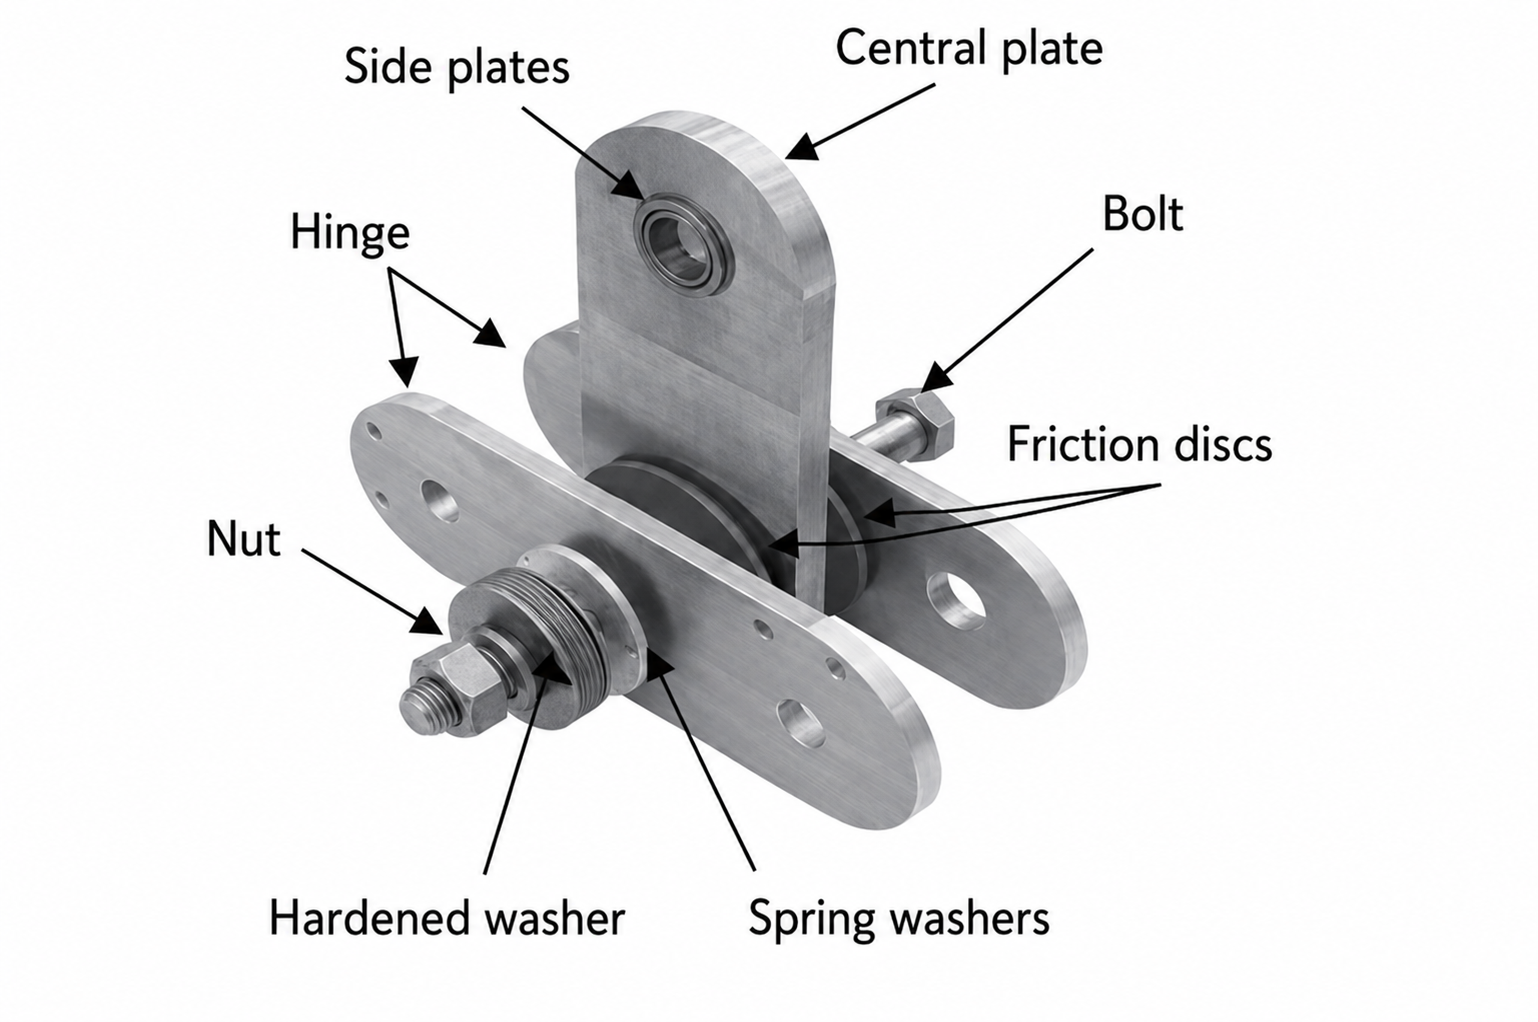
\includegraphics[width=\textwidth]{rfd_componentes.png}
        \caption{RFD components: central plate, lateral plates,
                 friction disks, prestressed bolt, and washers.}
        \label{fig:rfd_componentes}
    \end{subfigure}
    \hfill
    \begin{subfigure}[b]{0.48\textwidth}
        \centering
        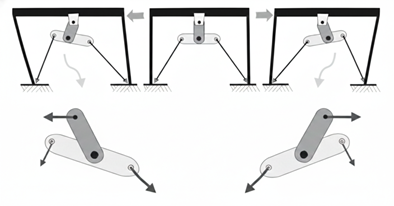
\includegraphics[width=\textwidth]{rfd_mecanismo.png}
        \caption{Actuation mechanism: lateral frame displacement induces
                 rotation in the device, dissipating energy through friction.}
        \label{fig:rfd_mecanismo}
    \end{subfigure}
    \caption{Rotational Friction Damper (RFD). Left: physical device configuration \citep{Mualla2002}.
             Right: activation sequence under lateral seismic excitation.}
    \label{fig:rfd}
\end{figure}

In a typical installation, the central plate connects to the beam midspan via a pin,
and the lateral plates attach to an inverted-V brace. When the frame drifts laterally,
relative inter-story motion rotates the device (Figure~\ref{fig:rfd_mecanismo}),
causing sliding between the steel plates and friction disks. This generates a resisting
moment that opposes motion, transferring energy away from the primary frame members and
into the friction mechanism \citep{kim_use_2011}.

The friction capacity is characterized by the maximum frictional moment $\Mf$, which
depends on the applied normal force, the friction coefficient, and the device geometry.
The equivalent lateral force transmitted to the frame is:
\begin{equation}
    F_{\mathrm{afr}} = \frac{\Mf}{\ha},
    \label{eq:Fafr}
\end{equation}
where $\ha$ is the lever arm of the bracing system. \citet{Mualla2002} found that the
moment-rotation behavior is nearly independent of frequency in the 2--7\,Hz range,
supporting use of Coulomb's friction law.

\subsection{Nonlinear Dynamic Analysis via Nonsmooth Dynamics}
\label{sec:theory:dns}

Coulomb friction complicates numerical integration because device behavior switches
abruptly between slip ($|\dot{\varphi}|>0$) and stick ($\dot{\varphi}=0$) with no
smooth transition. Standard step-by-step integrators assume forces vary smoothly
between time steps, an assumption that fails for dry friction
\citep{chopra_dynamics_2015}. To handle this without equivalent linearization, this
work uses the NSD method of \citet{Namorado2024}, which formulates the problem in
terms of velocities and impulses rather than accelerations and instantaneous forces.

\subsubsection*{Friction law}

For an RFD installed between stories $i$ and $i+1$, the resisting moment and the
relative angular velocity $\dot{\varphi}_i$ follow Coulomb's law:
\begin{equation}
    M_{\mathrm{afr},i} \in -\Mf \cdot \operatorname{Sign}\!\left(\dot{\varphi}_i\right),
    \label{eq:coulomb}
\end{equation}
where $\operatorname{Sign}(\cdot)$ is the extended sign operator:
\begin{equation}
    \operatorname{Sign}(v) =
    \begin{cases}
        \{+1\}    & \text{if } v > 0, \\
        [-1,\,+1] & \text{if } v = 0, \\
        \{-1\}    & \text{if } v < 0.
    \end{cases}
    \label{eq:sign}
\end{equation}
During slip ($|\dot{\varphi}_i|>0$), the moment equals exactly $\pm\Mf$. During
stick ($\dot{\varphi}_i=0$), the moment can take any value in $[-\Mf,\,+\Mf]$ as
required by static equilibrium.

\subsubsection*{Equation of motion}

The system of $\np$ stories with $n_a$ installed dampers is governed by the
differential inclusion \citep{Namorado2024}:
\begin{equation}
    \bm{M}\,\ddot{\bm{u}} + \bm{C}\,\dot{\bm{u}} + \bm{K}\,\bm{u}
    \in -\bm{M}\,\bm{r}\,\ddot{x}_g(t) + \bm{H}\,\bm{Q}_f(t),
    \label{eq:eom}
\end{equation}
where $\bm{M}$, $\bm{C}$, and $\bm{K}$ are the mass, damping, and stiffness
matrices; $\bm{u}$ is the vector of ground-relative displacements; $\bm{r}$ is the
seismic influence vector; $\ddot{x}_g$ is ground acceleration; and $\bm{H}$ is a
localization matrix (+1 on the upper story, $-1$ on the lower). The symbol $\in$
reflects that the friction force $\bm{Q}_f(t)$ is multivalued: it equals
$\pm\Mf/\ha$ during slip and can take any value in $[-\Mf/\ha,\,+\Mf/\ha]$ during
stick, consistent with Eq.~\ref{eq:coulomb}.

In the discrete implementation, the multivalued force $\bm{Q}_f$ is replaced by
frictional impulses $\bm{\lambda}_{k+1}$ computed at each step by solving a Linear
Complementarity Problem (LCP, Eq.~\ref{eq:lcp}). Once $\bm{\lambda}_{k+1}$ is found,
the force is uniquely determined for that step and the inclusion becomes an equality:
\begin{equation}
    \bm{M}\,\ddot{\bm{u}} + \bm{C}\,\dot{\bm{u}} + \bm{K}\,\bm{u}
    = -\bm{M}\,\bm{r}\,\ddot{x}_g(t) + \bm{H}\,\bm{\lambda}_{k+1}/\Delta t.
    \label{eq:eom_disc}
\end{equation}
The frictional force at story $i$ is then recovered as
$f_{\mathrm{afr},i} = \lambda_i / (\ha\,\Delta t)$.

\subsubsection*{NSD-LCP-PSOR Integration Procedure}

Starting from the known state at step $k$, the algorithm computes the state at $k+1$
in three steps, summarized in Algorithm~\ref{alg:nsd-lcp-psor}.

\textbf{Predictor.}
The velocity the system would have if dampers exerted no force is computed first.
A modified mass matrix is defined:
\begin{equation}
    \hat{\bm{M}} = \bm{M}
                  + \theta\Delta t\,\bm{C}
                  + (\theta\Delta t)^{2}\bm{K},
    \label{eq:Mhat}
\end{equation}
which combines inertia, damping, and stiffness into a single discrete operator.
The friction-free velocity is:
\begin{equation}
    \dot{\bm{u}}^{\mathrm{libre}} = \hat{\bm{M}}^{-1}
    \!\left[
        \bm{A}\,\dot{\bm{u}}_k
        - \Delta t\,\bm{K}\bm{u}_k
        - \theta\Delta t\,\bm{M}\!\left(\ddot{x}_{g,k+1}+\ddot{x}_{g,k}\right)\bm{r}
    \right],
    \label{eq:vfree}
\end{equation}
where $\bm{A} = \bm{M} - \theta\Delta t\,\bm{C} - (\theta\Delta t)^{2}\bm{K}$.
This is equivalent to standard Newmark integration without friction.

\textbf{Corrector.}
In general, the free velocity does not satisfy Coulomb's condition: some dampers show
nonzero relative velocity when they should be at rest. The corrector finds the
frictional impulses $\bm{\lambda}_{k+1}$ that satisfy both system dynamics and
Coulomb's constraints. The free relative velocity at each damper is
$q_r = \dot{u}^{\mathrm{libre}}_{f_r} - \dot{u}^{\mathrm{libre}}_{f_r-1}$, and the
coupling matrix between devices is:
\begin{equation}
    W_{rs} = \left[\bm{H}^{\top}\hat{\bm{M}}^{-1}\bm{H}\right]_{rs}\Delta t,
    \label{eq:W}
\end{equation}
whose entries describe how the impulse of one damper affects the relative velocity of
others through the structure. The impulses are found by solving:
\begin{equation}
    \bm{W}\bm{\lambda} + \bm{q} = \bm{0},
    \quad |\lambda_r| \leq \frac{\Mf\,\Delta t}{\ha},
    \quad r = 1,\ldots,n_a,
    \label{eq:lcp}
\end{equation}
which is an LCP with box constraints. When a damper's impulse reaches $\Mf\Delta t/\ha$,
the device is slipping; when below, it is stuck. The system is solved iteratively via
PSOR (\textit{Projected Successive Over-Relaxation}), updating each impulse in sequence
and projecting it onto the admissible interval until convergence.

\textbf{State update.}
With the computed impulses, the velocity is corrected and displacement is advanced:
\begin{align}
    \dot{\bm{u}}_{k+1} &= \dot{\bm{u}}^{\mathrm{libre}}
        + \Delta t\,\hat{\bm{M}}^{-1}\bm{H}\bm{\lambda}_{k+1}, \label{eq:vupdate}\\
    \bm{u}_{k+1} &= \bm{u}_k
        + \Delta t\!\left[(1-\theta)\,\dot{\bm{u}}_k
                         + \theta\,\dot{\bm{u}}_{k+1}\right]. \label{eq:uupdate}
\end{align}
The impulse $\bm{\lambda}_{k+1}$ is reused as the starting point for PSOR in the next
step, exploiting the fact that the friction response changes little between consecutive
instants.

\begin{algorithm}[t]
\caption{NSD-LCP-PSOR applied to MDOF frames with RFD}
\label{alg:nsd-lcp-psor}
\begin{algorithmic}[1]
\Require $\bm{M},\bm{C},\bm{K}$; $\bm{H}$, $\bm{F}^{\lim}$;
         $\{\ddot{x}_{g,k}\}_{k=0}^{n}$; $\Delta t$, $\theta$
\Ensure  $\{\bm{u}_k,\dot{\bm{u}}_k\}_{k=0}^{n}$

\vspace{2pt}
\State \textit{// Pre-computation (once only)}
\State $\hat{\bm{M}} \leftarrow \bm{M} + \theta\Delta t\,\bm{C} + (\theta\Delta t)^{2}\bm{K}$
\State $\bm{A} \leftarrow \bm{M} - \theta\Delta t\,\bm{C} - (\theta\Delta t)^{2}\bm{K}$
\State $\bm{W} \leftarrow \left(\bm{H}^{\top}\hat{\bm{M}}^{-1}\bm{H}\right)\Delta t$
\State $\bm{u}_0 \leftarrow \bm{0}$;\quad $\dot{\bm{u}}_0 \leftarrow \bm{0}$;\quad
       $\bm{\lambda}_0 \leftarrow \bm{0}$

\vspace{2pt}
\For{$k = 0, 1, \ldots, n-1$}
    \vspace{2pt}
    \State \textit{// Step 1 — free velocity (friction-free predictor)}
    \State $\bm{b}_k \leftarrow \bm{A}\,\dot{\bm{u}}_k
            - \Delta t\,\bm{K}\bm{u}_k
            - \theta\Delta t\,\bm{M}
              \!\left(\ddot{x}_{g,k+1}+\ddot{x}_{g,k}\right)\bm{r}$
    \State $\dot{\bm{u}}^{\mathrm{lib}} \leftarrow \hat{\bm{M}}^{-1}\bm{b}_k$

    \vspace{2pt}
    \State \textit{// Step 2 — free relative velocities at each damper}
    \State $q_r \leftarrow \dot{u}^{\mathrm{lib}}_{f_r} - \dot{u}^{\mathrm{lib}}_{f_r-1}$
           \quad for $r = 1,\ldots,n_a$

    \vspace{2pt}
    \State \textit{// Step 3 — LCP resolution via PSOR (corrector)}
    \State $\bm{\lambda}^{(0)} \leftarrow \bm{\lambda}_k$
           \quad\textit{(starting point from previous step)}
    \While{$\|\bm{\lambda}^{(i+1)} - \bm{\lambda}^{(i)}\|_\infty > \varepsilon$}
        \For{$r = 1,\ldots,n_a$}
            \State $\tilde{\lambda}_r \leftarrow
                   -\!\left(q_r + \sum_{s \neq r} W_{rs}\lambda_s^{(i)}\right)\!\big/W_{rr}$
            \State $\lambda_r^{(i+1)} \leftarrow
                   \max\!\left(-F^{\lim}_r,\;\min\!\left(F^{\lim}_r,\;\tilde{\lambda}_r\right)\right)$
        \EndFor
    \EndWhile
    \State $\bm{\lambda}_{k+1} \leftarrow \bm{\lambda}^{(*)}$
           \quad\textit{($F^{\lim}_r = \Mf\Delta t/\ha$)}

    \vspace{2pt}
    \State \textit{// Step 4 — state update}
    \State $\dot{\bm{u}}_{k+1} \leftarrow
           \dot{\bm{u}}^{\mathrm{lib}} +
           \Delta t\,\hat{\bm{M}}^{-1}\bm{H}\bm{\lambda}_{k+1}$
    \State $\bm{u}_{k+1} \leftarrow \bm{u}_k +
           \Delta t\!\left[(1-\theta)\,\dot{\bm{u}}_k +
                           \theta\,\dot{\bm{u}}_{k+1}\right]$
\EndFor
\end{algorithmic}
\end{algorithm}

The time step $\Delta t = 0.01$\,s matches the native sampling interval of the seismic
records, avoiding interpolation of the input signal. For the stiffest structures in the
experiment ($T_1 = 0.3$\,s), this gives approximately 30 integration points per period,
satisfying the standard criterion $\Delta t / T_1 \leq 0.10$ for Newmark methods
\citep{chopra_dynamics_2015}. The frictional force at story $i$ is recovered as:
\begin{equation}
    f_{\mathrm{afr},i} = \frac{\lambda_i}{\ha\,\Delta t},
    \label{eq:ffrict}
\end{equation}
so the stick or slip state of each device is determined automatically by the LCP
solution, with no explicit detection logic.

\subsubsection*{Adaptation of NSD Method for Massive MDOF Simulation}
\label{sec:theory:nsd:adaptacion}

The NSD method of \citet{Namorado2024} was validated for frames of one to five stories
with one damper per story. This work extends it to frames of up to twenty stories with
variable damper configurations, requiring three adjustments.

\textbf{LCP formulation of the corrector.}
Instead of updating each damper's impulse separately, all are solved jointly through the
matrix $\bm{W}$ (Eq.~\ref{eq:W}), which captures the interaction between devices through
the structure. This is more direct when multiple dampers are active simultaneously on
different stories, though it requires computing $\hat{\bm{M}}^{-1}$ once before
integration begins.

\textbf{No tuning parameter.}
The original algorithm includes a parameter $\alpha$ that controls corrector convergence
speed and must be chosen case by case. Formulating the problem as an LCP eliminates this
parameter: the iterative procedure converges without manual tuning, which is critical when
running thousands of distinct configurations.

\textbf{Impulse reuse between steps.}
The impulse from step $k$ is used as the starting point at step $k+1$. Because the
structural response changes gradually, this warm start is close to the solution and
requires fewer PSOR iterations.

In physical terms, both formulations solve the same discrete Coulomb friction law. The
difference is computational organization, adapted here to handle larger buildings and more
dampers efficiently.

\subsection{Seismic Performance Metric}
\label{sec:theory:metrica}

Seismic performance is quantified using normalized response ratios relative to the bare
frame, consistent with prior RFD studies
\citep{Namorado2024, Jarrahi2020jbe, Mualla2002}. For each configuration--record pair,
three ratios are computed:
\begin{equation}
    R_1 = \frac{u_{\max}^{(c)}}{u_{\max}^{(0)}}, \quad
    R_2 = \frac{\ddot{u}_{\max}^{(c)}}{\ddot{u}_{\max}^{(0)}}, \quad
    R_3 = \frac{V_{\max}^{(c)}}{V_{\max}^{(0)}},
    \label{eq:R_individual}
\end{equation}
where superscripts (c) and (0) denote controlled and uncontrolled structures; $u_{\max}$
is maximum roof displacement, $\ddot{u}_{\max}$ is maximum absolute acceleration, and
$V_{\max}$ is maximum base shear. Two composite indices are built using the Euclidean
norm. The first combines displacement and acceleration:
\begin{equation}
    CR_1 = \sqrt{R_1^2 + R_2^2},
    \label{eq:CR1}
\end{equation}
and the second adds base shear to include all three response aspects:
\begin{equation}
    CR_2 = \sqrt{R_1^2 + R_2^2 + R_3^2}.
    \label{eq:CR2}
\end{equation}
When dampers have no effect, $R_1 = R_2 = R_3 = 1$ and $CR_2 = \sqrt{3}$. Smaller
values indicate improved seismic performance.

Because seismic response depends on the ground motion record, $CR_2$ is summarized
across $N_r = 8$ records using three percentile statistics, following standard practice
in performance-based evaluation \citep{Kazemi2022}:
\begin{align}
    \CR{P10} &= Q_{0.10}\!\left(\{CR_2^{(k)}\}_{k=1}^{N_r}\right), \quad
    \CR{med}  = Q_{0.50}\!\left(\{CR_2^{(k)}\}_{k=1}^{N_r}\right), \notag\\
    \CR{P90} &= Q_{0.90}\!\left(\{CR_2^{(k)}\}_{k=1}^{N_r}\right),
    \label{eq:CR2stats}
\end{align}
where $Q_p$ denotes the $p$-th quantile. These three statistics are the target variables
for the ML models. $\CR{P10}$ represents a favorable condition, $\CR{med}$ describes
typical behavior, and $\CR{P90}$ approximates a severe condition within the record set.
Together, they distinguish configurations that only perform well under a single record
from those that are robust across seismic variability.

\subsection{Machine Learning for Structural Optimization}
\label{sec:theory:ml}

Optimizing passive dissipation systems means finding the best combination of device
location, count, and capacity to minimize seismic response. Prior work used energy
methods and metaheuristic algorithms for this purpose
\citep{moreschi_design_2003, moghaddam_optimal_2022, ontiveros-perez_reliability-based_2019}.
ML enables surrogate models that approximate the input--output mapping of nonlinear
analysis at much lower cost, enabling efficient exploration of high-dimensional design
spaces.

In the surrogate paradigm, a regression function $\hat{y} = f(\bm{x};\,\bm{\theta})$
is trained on data $\{(\bm{x}_i,\,y_i)\}_{i=1}^{N}$ to map design variables $\bm{x}$
(structural and RFD parameters) to a target $y$ (one of the three $CR_2$ statistics).
Training minimizes mean squared error:
\begin{equation}
    \mathcal{L}(\bm{\theta}) = \frac{1}{N}\sum_{i=1}^{N}
    \bigl(y_i - f(\bm{x}_i;\,\bm{\theta})\bigr)^2.
    \label{eq:mse}
\end{equation}

Four algorithms are compared: (i)~Linear Regression and (ii)~Ridge Regression
($\ell_2$ penalization) as linear baselines; (iii)~Random Forest \citep{Breiman2001},
which averages predictions from many independently-trained trees; and (iv)~XGBoost
\citep{Chen2016}, a gradient boosting algorithm that sequentially corrects the residuals
of a growing ensemble. Generalization is estimated via five-fold GroupKFold
cross-validation \citep{Kazemi2022}, where groups are unique structure identifiers. This
prevents different configurations of the same building---which share dynamic properties
and therefore have correlated responses---from appearing in both training and validation
folds, avoiding information leakage. Evaluation metrics are:
\begin{equation}
    \RMSE = \sqrt{\frac{1}{|V|}\sum_{i \in V}\bigl(y_i - \hat{y}_i\bigr)^2},
    \qquad
    \Rsq  = 1 - \frac{\sum_{i \in V}(y_i - \hat{y}_i)^2}
                      {\sum_{i \in V}(y_i - \bar{y})^2},
    \label{eq:metrics}
\end{equation}
where $V$ is the validation set, $\hat{y}_i$ are out-of-fold predictions, and $\bar{y}$
is the mean of observed values.

%%═══════════════════════════════════════════════════════════════════════════
\section{Methodology}
\label{sec:method}
%%═══════════════════════════════════════════════════════════════════════════

\subsection{Design of Experiments}
\label{sec:method:doe}

Latin Hypercube Sampling (LHS) \citep{McKay1979} was used to generate 1,000
structurally diverse shear-type frames. Each configuration is defined by five
structural variables: number of stories $\np \in \{3, 5, 7, 10, 12, 15, 18, 20\}$;
target fundamental period $T_1 \in [0.3,\,3.0]$\,s; average mass per level
$\bar{m} \in [150,\,350]$\,t/story; mass distribution profile (uniform, linear
ascending, linear descending, or concentrated at top); and lateral stiffness profile
(uniform, linear ascending, linear descending, or soft story at base). Lateral stiffness
was analytically calibrated to meet the target $T_1$ via the generalized eigenvalue
problem $(\bm{K} - \omega_1^2\,\bm{M})\,\bm{\phi}_1 = \bm{0}$, with $\omega_1 = 2\pi/T_1$.

For each structure, approximately 50 RFD configurations were generated: 40 via LHS over
the binary location space and frictional moment range $\Mf \in [25,\,500]$\KM, and 10
structured configurations targeting specific coverage fractions. The configuration is
encoded by a binary vector $\bm{b} \in \{0,1\}^{\np}$, where $b_i = 1$ means an RFD is
installed at story $i$. This yields device count $\nd = \|\bm{b}\|_0$ and coverage density
$\etad = \nd/\np \in (0,\,1]$. The full plan comprises 433,984 simulations
($\approx 1,000 \times 54 \times 8$).

\subsection{Structural Models and Dynamic Analysis}
\label{sec:method:modelo}

Each structure is modeled as a linear shear frame with concentrated masses per story and
lateral stiffness between stories. The diagonal mass matrix is
$\bm{M} = \mathrm{diag}(m_1,\ldots,m_{\np})$ and the tridiagonal stiffness matrix
$\bm{K}$ is assembled from the inter-story stiffness vector $k_i$. Rayleigh damping
is used with ratio $\zeta = 3\%$, calibrated to modes 1 and 3
\citep{chopra_dynamics_2015}. The eight real accelerograms are: El~Centro~1940,
Jamiltepec~2018, Kobe~1995, Loma Prieta~1989, Niltepec~2017, Northridge~1994,
Trinidad~1983, and Zacatula~1997. Time-history integration follows the NSD midpoint
scheme \citep{Namorado2024} with $\Delta t = 0.01$\,s, equal to the native sampling
interval. The lever arm is fixed at $\ha = 0.40$\,m, within the range reported for
steel frames with RFDs \citep{Mualla2002, Jarrahi2020jbe}.

\subsection{Feature Engineering}
\label{sec:method:features}

The four primary design variables do not capture the spatial distribution of RFDs or
the scaling relations between parameters. A tree-based model trained only on them would
need to infer ratios and positions from raw components, increasing required tree depth
and potentially reducing generalization. Five derived features are therefore added to
encode this information explicitly.

The complete feature vector contains 29 predictors in three groups:

\begin{enumerate}[label=\textit{\roman*})]
    \item \textbf{Primary design variables} (4):
          number of stories $\np$, target fundamental period $T_1$,
          frictional moment $\Mf$, and damper count $\nd$.

    \item \textbf{Derived features} (5):
    \begin{itemize}
        \item $\etad = \nd/\np$: damper density, the dominant design variable per
              importance analysis (Section~\ref{sec:results:importancia});
        \item $\bar{p} = \tfrac{1}{\nd}\sum_{i:\,b_i=1} i$: mean device position in
              story number;
        \item $\tilde{p} = \bar{p}/\np \in (0,\,1]$: normalized mean position,
              indicating whether RFDs are concentrated in lower or upper stories;
        \item $\sigma_p = \mathrm{std}\!\left(\{i:b_i=1\}\right)/\np$: normalized
              vertical dispersion, distinguishing uniform from clustered configurations;
        \item $\tilde{E} = E_{\mathrm{total}}/(\np\times10^6)$: total dissipated
              energy normalized by number of stories, a proxy for integrated dynamic
              demand.
    \end{itemize}

    \item \textbf{Binary location indicators} (20):
          $b_1,\ldots,b_{20}$, where $b_i=1$ if story $i$ has an RFD and $b_i=0$
          otherwise; frames with fewer than 20 stories are padded with zeros.
\end{enumerate}

\subsection{Training and Validation}
\label{sec:method:entrenamiento}

The objectives $\CR{med}$, $\CR{P10}$, and $\CR{P90}$ are predicted independently.
For each objective, all four algorithms are trained and evaluated via five-fold
GroupKFold cross-validation. Hyperparameters are fixed to standard values: Random
Forest uses $n=100$ trees and maximum depth 15; XGBoost uses $n=100$ estimators,
maximum depth 6, and learning rate $\eta=0.1$. Feature importance is computed from
mean impurity decrease across all trees in the trained XGBoost model. Out-of-fold
(OOF) predictions are assembled across folds to compute the reported $\RMSE$ and
$\Rsq$ values.

%%═══════════════════════════════════════════════════════════════════════════
\section{Results}
\label{sec:results}
%%═══════════════════════════════════════════════════════════════════════════

\subsection{Predictive Performance of ML Models}
\label{sec:results:desempenio}

Table~\ref{tab:desempenio} shows RMSE and $R^2$ with cross-validation for all models
and objectives. Ensemble models achieve a 49\% reduction in $\RMSE$ relative to linear
baselines for $\CR{med}$, and 40\% for $\CR{P10}$. XGBoost gives the lowest error for
$\CR{med}$ and $\CR{P10}$, while Random Forest shows a slight advantage for $\CR{P90}$
(\cref{fig:comparacion_modelos}).

\begin{table}[h!]
\centering
\caption{RMSE and $R^2$ with cross-validation by model and target variable.
         Five-fold GroupKFold, grouped by structure identifier.}
\label{tab:desempenio}
\small
\setlength{\tabcolsep}{4pt}
\begin{tabular}{lcccccc}
\toprule
& \multicolumn{2}{c}{$\CR{med}$}
& \multicolumn{2}{c}{$\CR{P10}$}
& \multicolumn{2}{c}{$\CR{P90}$} \\
\cmidrule(lr){2-3}\cmidrule(lr){4-5}\cmidrule(lr){6-7}
Model & $\RMSE$ & $\Rsq$ & $\RMSE$ & $\Rsq$ & $\RMSE$ & $\Rsq$ \\
\midrule
Linear Regression & 0.1274 & 0.695 & 0.1267 & 0.812 & 0.1838 & 0.435 \\
Ridge            & 0.1274 & 0.695 & 0.1268 & 0.812 & 0.1838 & 0.435 \\
Random Forest    & 0.0681 & 0.913 & 0.0785 & 0.928 & 0.0981 & \textbf{0.839} \\
XGBoost          & \textbf{0.0652} & \textbf{0.920} & \textbf{0.0755} & \textbf{0.933} & 0.0984 & 0.838 \\
\bottomrule
\end{tabular}
\end{table}

\begin{figure}[htbp]
\centering
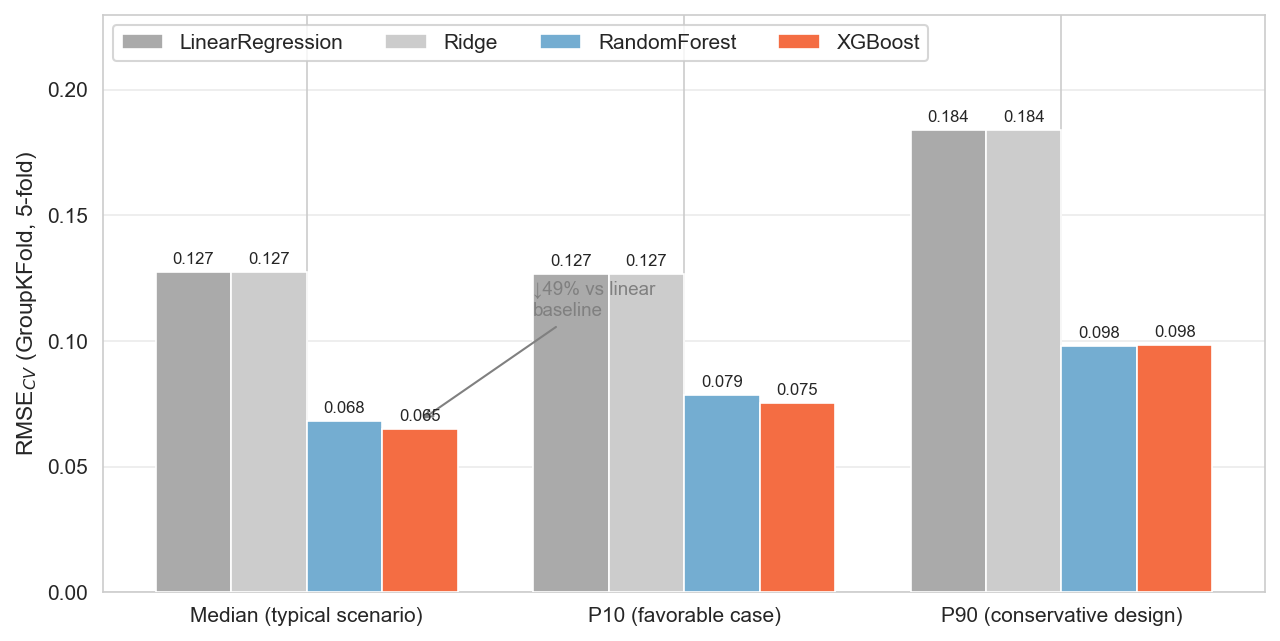
\includegraphics[width=0.85\linewidth]{figs/F1_model_comparison_rmse.png}
\caption{Comparison of cross-validation RMSE across models and target variables.
Ensemble models achieve approximately half the error of linear baselines.}
\label{fig:comparacion_modelos}
\end{figure}

For $\CR{P10}$, linear models reach $\Rsq = 0.81$, showing that the relationship
between predictors and response is largely linear in favorable scenarios. The much
lower $\Rsq = 0.44$ for $\CR{P90}$ under linear models confirms that the conservative
scenario is governed by nonlinear interactions that only ensemble models can capture.

\Cref{fig:pred_vs_actual} shows OOF scatter for XGBoost on $\CR{med}$ with residual
analysis. Predictions cluster tightly around the identity line with no systematic bias.
Residuals grow slightly for $CR_2 > 1.8$, a zone dominated by low-rise frames
($\np \leq 5$). In these cases, structural response is more sensitive to small
parameter changes, which increases target variability and makes prediction harder.

\begin{figure}[htbp]
\centering
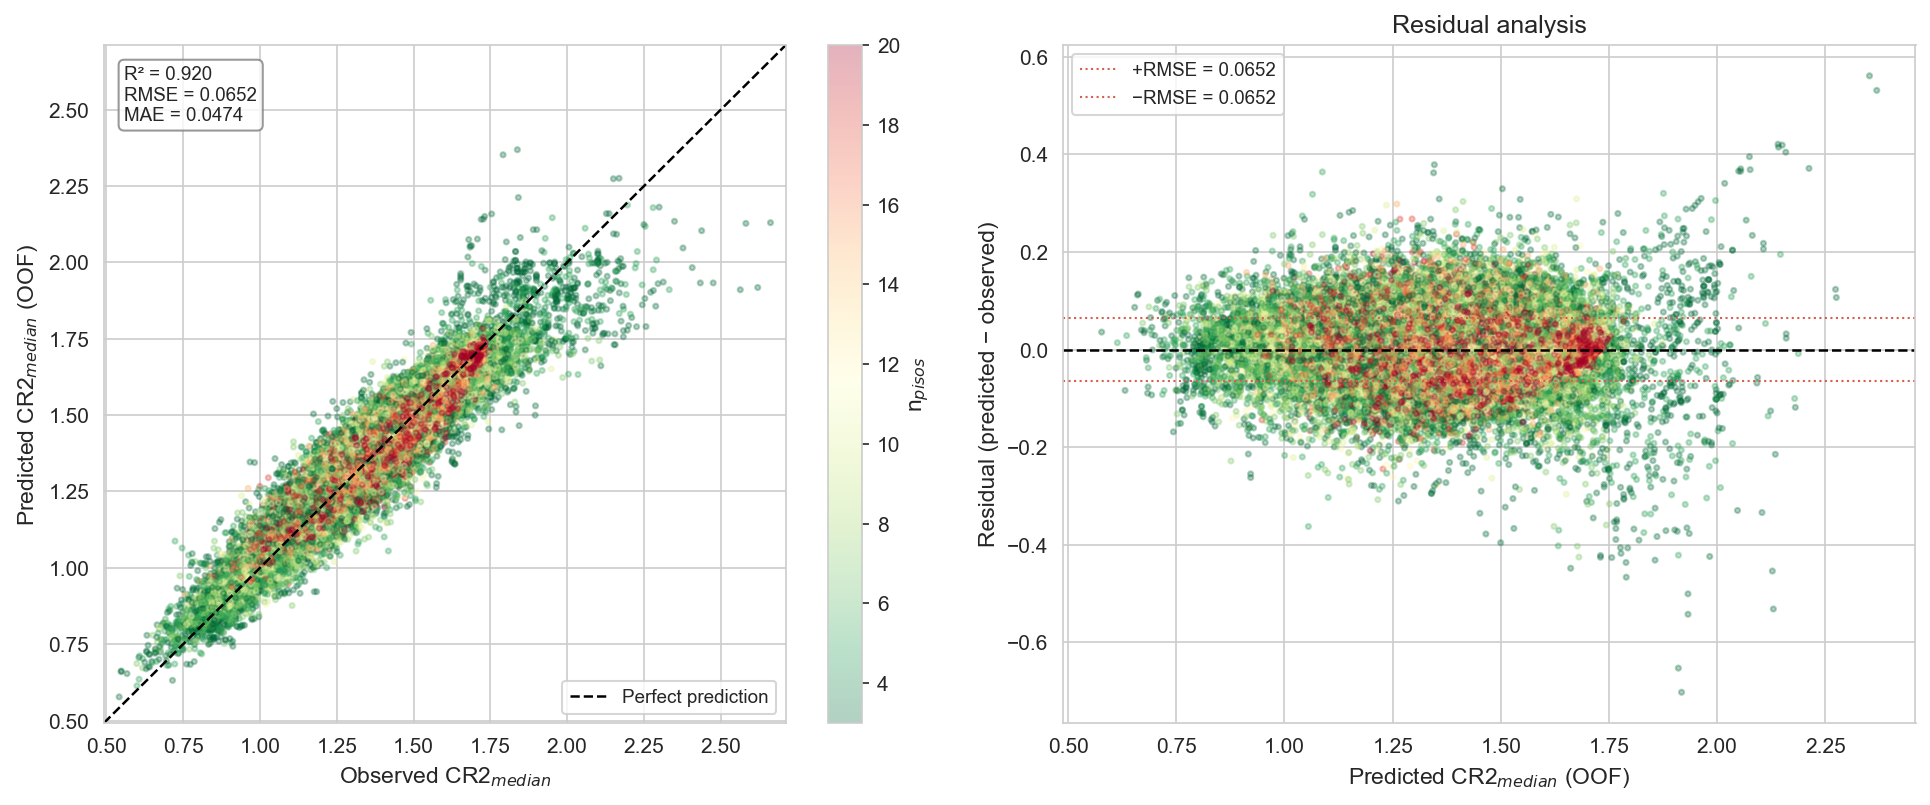
\includegraphics[width=\linewidth]{figs/F2_predicted_vs_actual_oof.png}
\caption{XGBoost OOF for $\CR{med}$. \textit{Left}: prediction vs.\ observed value;
dashed line: perfect prediction; color: $\np$. \textit{Right}: residuals (predicted $-$ observed)
vs.\ predicted; dashed bands: $\pm\RMSE$. $\Rsq = 0.92$, $\RMSE = 0.065$.}
\label{fig:pred_vs_actual}
\end{figure}

\begin{figure}[htbp]
\centering
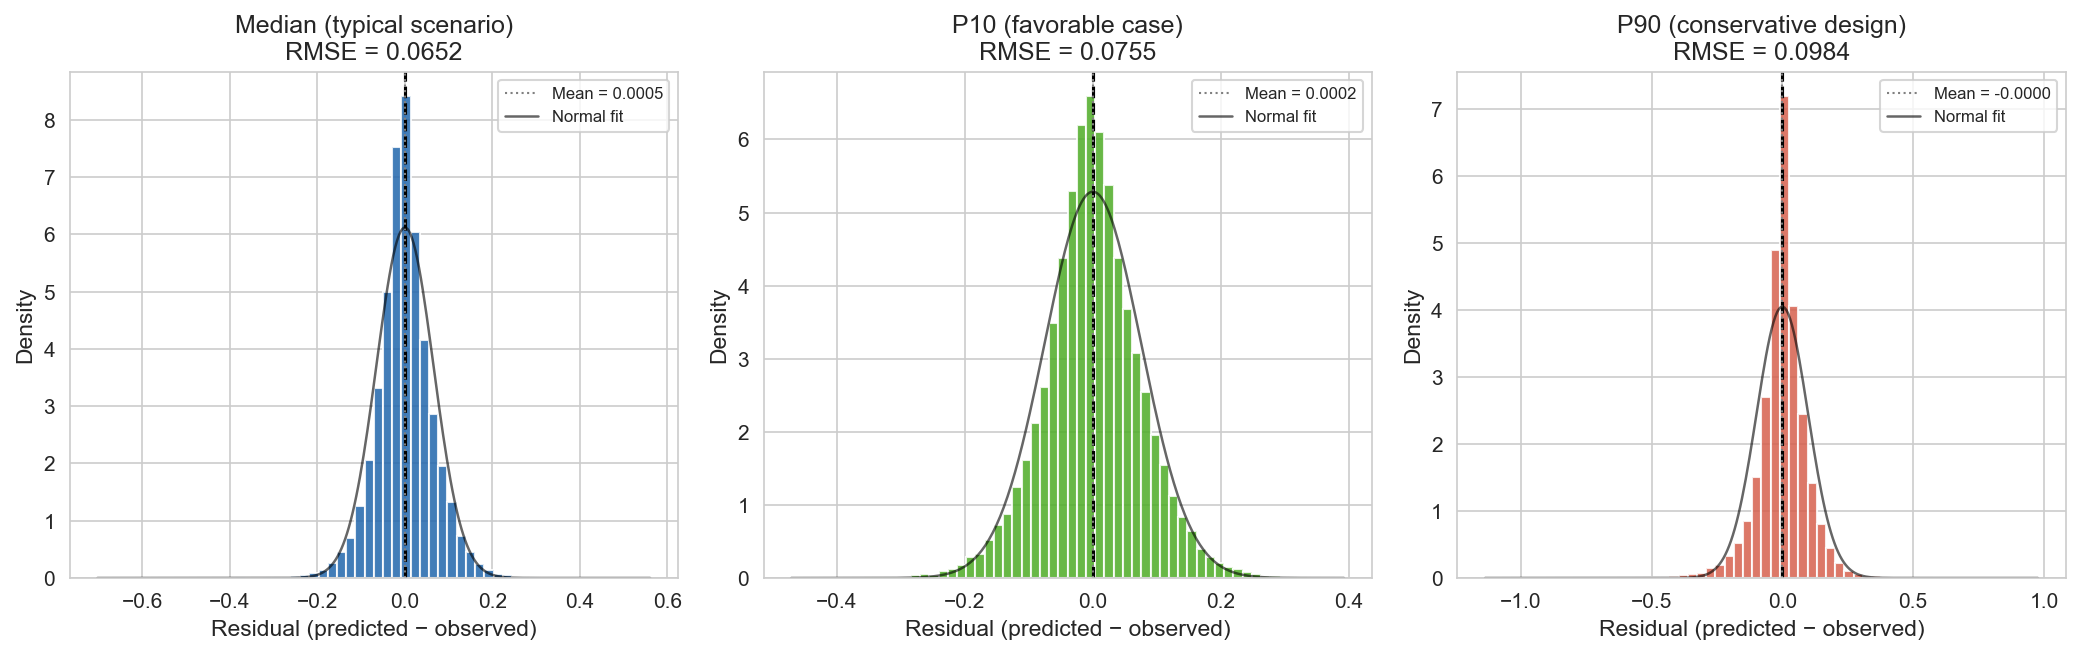
\includegraphics[width=\linewidth]{figs/F3_residual_distributions.png}
\caption{Residual distributions (OOF, XGBoost) for the three target variables of $CR_2$.
Dashed line: zero mean reference; solid curve: normal fit.}
\label{fig:residuales}
\end{figure}

\subsection{Design Variable Hierarchy and Feature Importance}
\label{sec:results:importancia}

Figure~\ref{fig:importancia} shows the top 12 features for each target variable from the
XGBoost model. Damper density $\etad$ ranks first across all three scenarios, with
Pearson correlation $r = -0.73$ with $\CR{med}$, versus $r = -0.45$ for absolute count
$\nd$.

Normalized dissipated energy $\tilde{E}$ ($r = -0.70$) and vertical dispersion
$\sigma_p$ ($r = -0.54$) rank second and third. These two are closely linked: a
homogeneous vertical distribution of devices promotes more uniform energy dissipation
across stories and reduces demand concentration at specific levels. Configurations that
include lower stories---where inter-story drift is typically largest---are more
efficient, consistent with \citet{aydin_simple_2013} and the optimization results of
\citet{moghaddam_optimal_2022} and \citet{miguel_simultaneous_2016}. Frictional moment
$\Mf$ shows weaker marginal correlation ($r = -0.19$) in isolation, but interacts
strongly with $\etad$, as shown in \cref{sec:results:interaccion}.

A notable difference between scenarios is the behavior of $\CR{P90}$: $\etad$ loses
its dominant rank (first for median and P10, fourth for P90) and is replaced by damper
presence at stories 1 and 2 and by building height $\np$, which occupy the top three
positions. Under the most demanding records, precise placement at lower levels and
structural characteristics matter more than global coverage.

\begin{figure}[htbp]
\centering
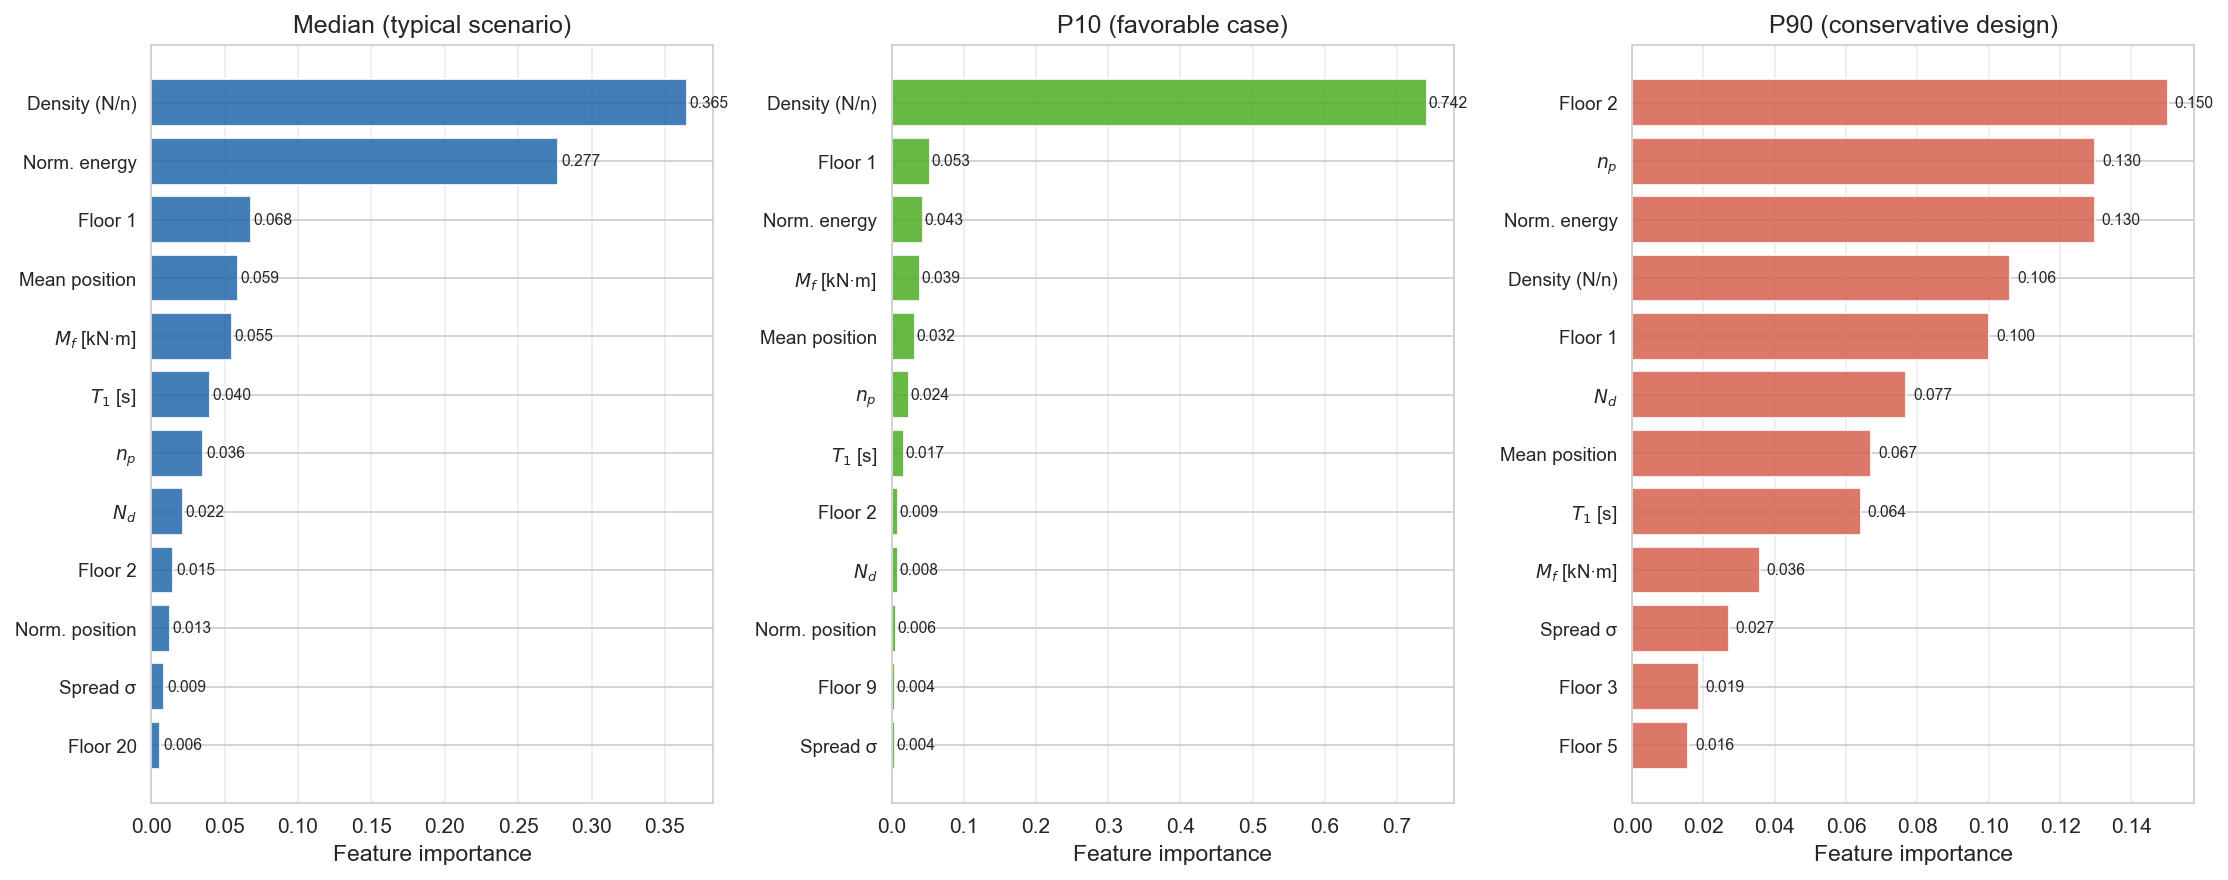
\includegraphics[width=\linewidth]{figs/F4_feature_importance_3targets.png}
\caption{Feature importance (XGBoost) for the top 12 predictors in the three $CR_2$ scenarios.
Horizontal bars indicate mean impurity decrease, normalized within each model. Note: horizontal axes
of each panel have independent scales; comparison between scenarios should be made by relative importance
rank, not absolute magnitude.}
\label{fig:importancia}
\end{figure}

\subsection{Diminishing Returns: Effect of Damper Density}
\label{sec:results:decreciente}

Figure~\ref{fig:decreciente} shows the diminishing returns relationship between $\etad$
and $CR_2$. For each structure, the best $\CR{med}$ achievable at each value of $\nd$
was identified by selecting the minimum $CR_2$ among all configurations with that count.
Curves are stratified by building height to remove the confounding effect of $\np$ on
the absolute $\nd$ axis.

All height categories show a consistent diminishing returns pattern. The steepest
improvement occurs in $\etad \in [0.30,\,0.60]$. Beyond $\etad = 0.60$, marginal gain
per additional story covered decreases monotonically. A threshold analysis based on
normalized within-structure gain (Figure~\ref{fig:curvas_internas}) shows that 80\% of
maximum performance improvement is reached at $\etad \approx 0.85$ for mid-rise
(6--10 stories), high-rise (11--15 stories), and tall (16--20 stories) frames. Low-rise
frames (3--5 stories) require $\etad \approx 0.95$ to reach the same 80\% threshold,
because each additional device has proportionally greater impact in short buildings.

To check whether $\etad$ dominance holds independent of other design variables,
stochastic dominance analysis was performed on each of the eight records separately.
On each record, the 5th percentile (best 5\%) of $CR_2$ in a higher density interval
was compared against the 95th percentile (worst 5\%) of the immediately lower interval.
Dominance is confirmed across all eight records: even an unfavorable configuration in
$\Mf$, position, or $T_1$, but with greater coverage density, outperforms 95\% of
configurations with lower density. Pearson correlation between $\etad$ and $CR_2$
ranges from $r=-0.74$ (El~Centro~1940) to $r=-0.55$ (Kobe~1995). The exception is
Trinidad~1983 ($r=-0.18$), where correlation with density weakens and position and
per-device capacity variables become more relevant, suggesting that low-intensity or
atypically-spectrummed records can reduce $\etad$ dominance.

\begin{figure}[htbp]
\centering
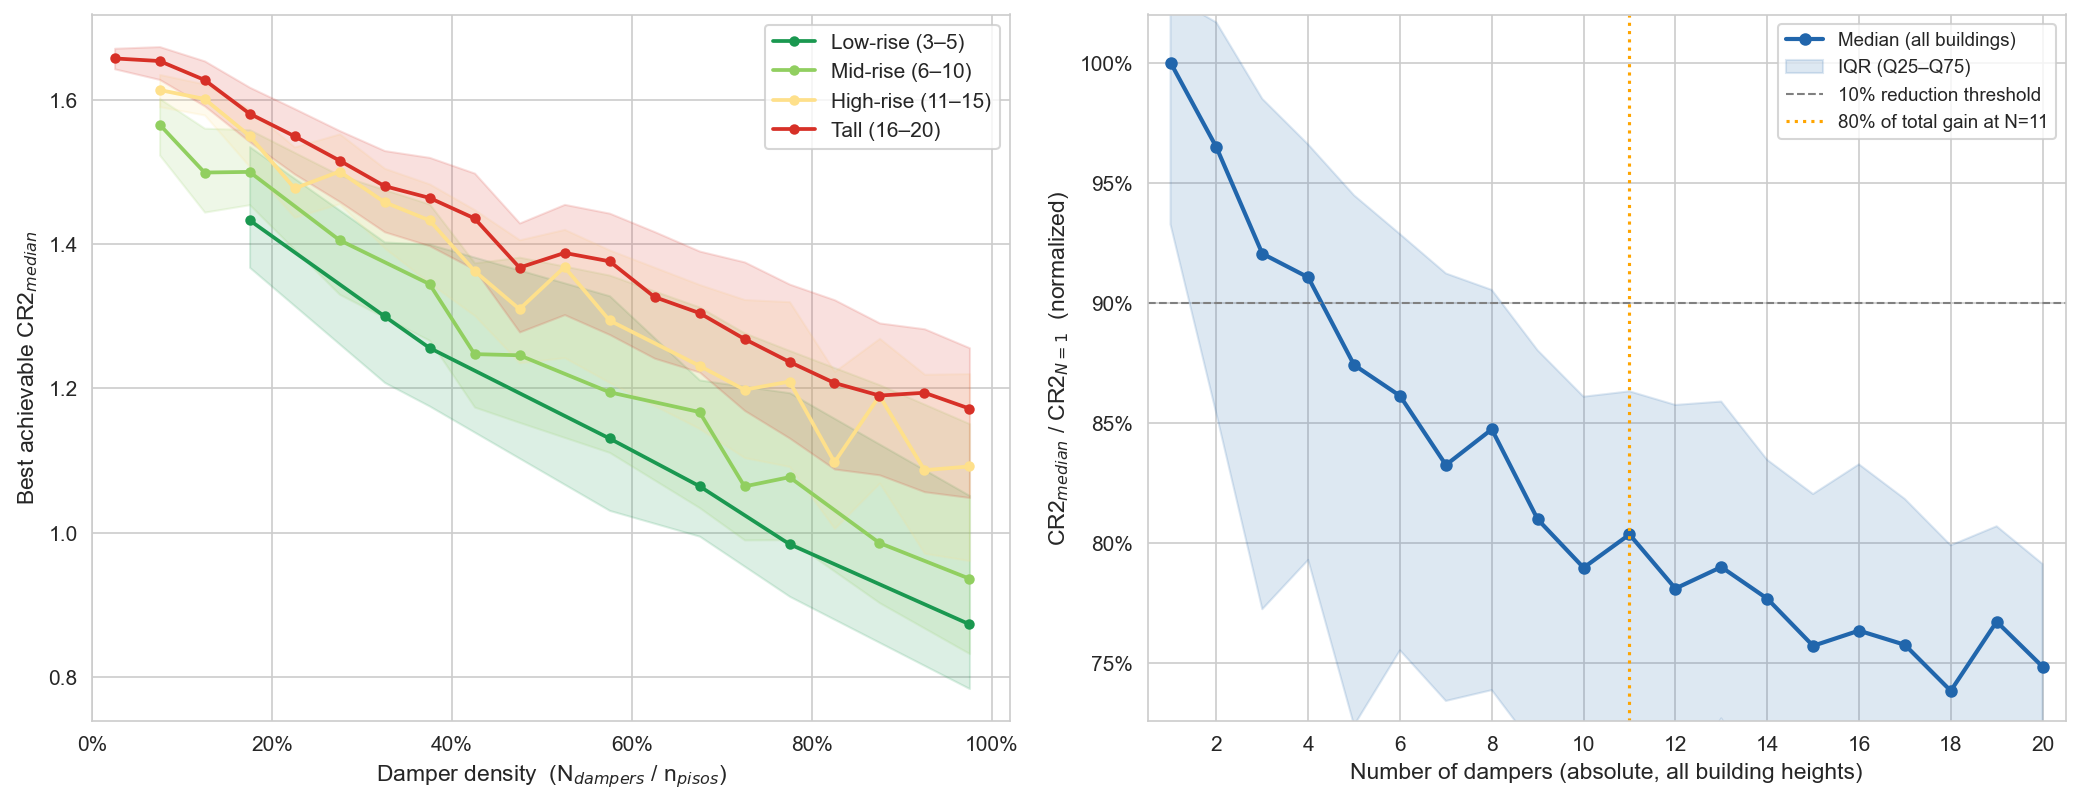
\includegraphics[width=\linewidth]{figs/F5_diminishing_returns.png}
\caption{Left: best achievable $\CR{med}$ vs.\ coverage density $\etad$, stratified by building height
(median $\pm$ IQR). Right: normalized $CR_2$ vs.\ absolute $\nd$ across all buildings (note: confounded
with height; left panel provides appropriate comparison).}
\label{fig:decreciente}
\end{figure}

\begin{figure}[htbp]
\centering
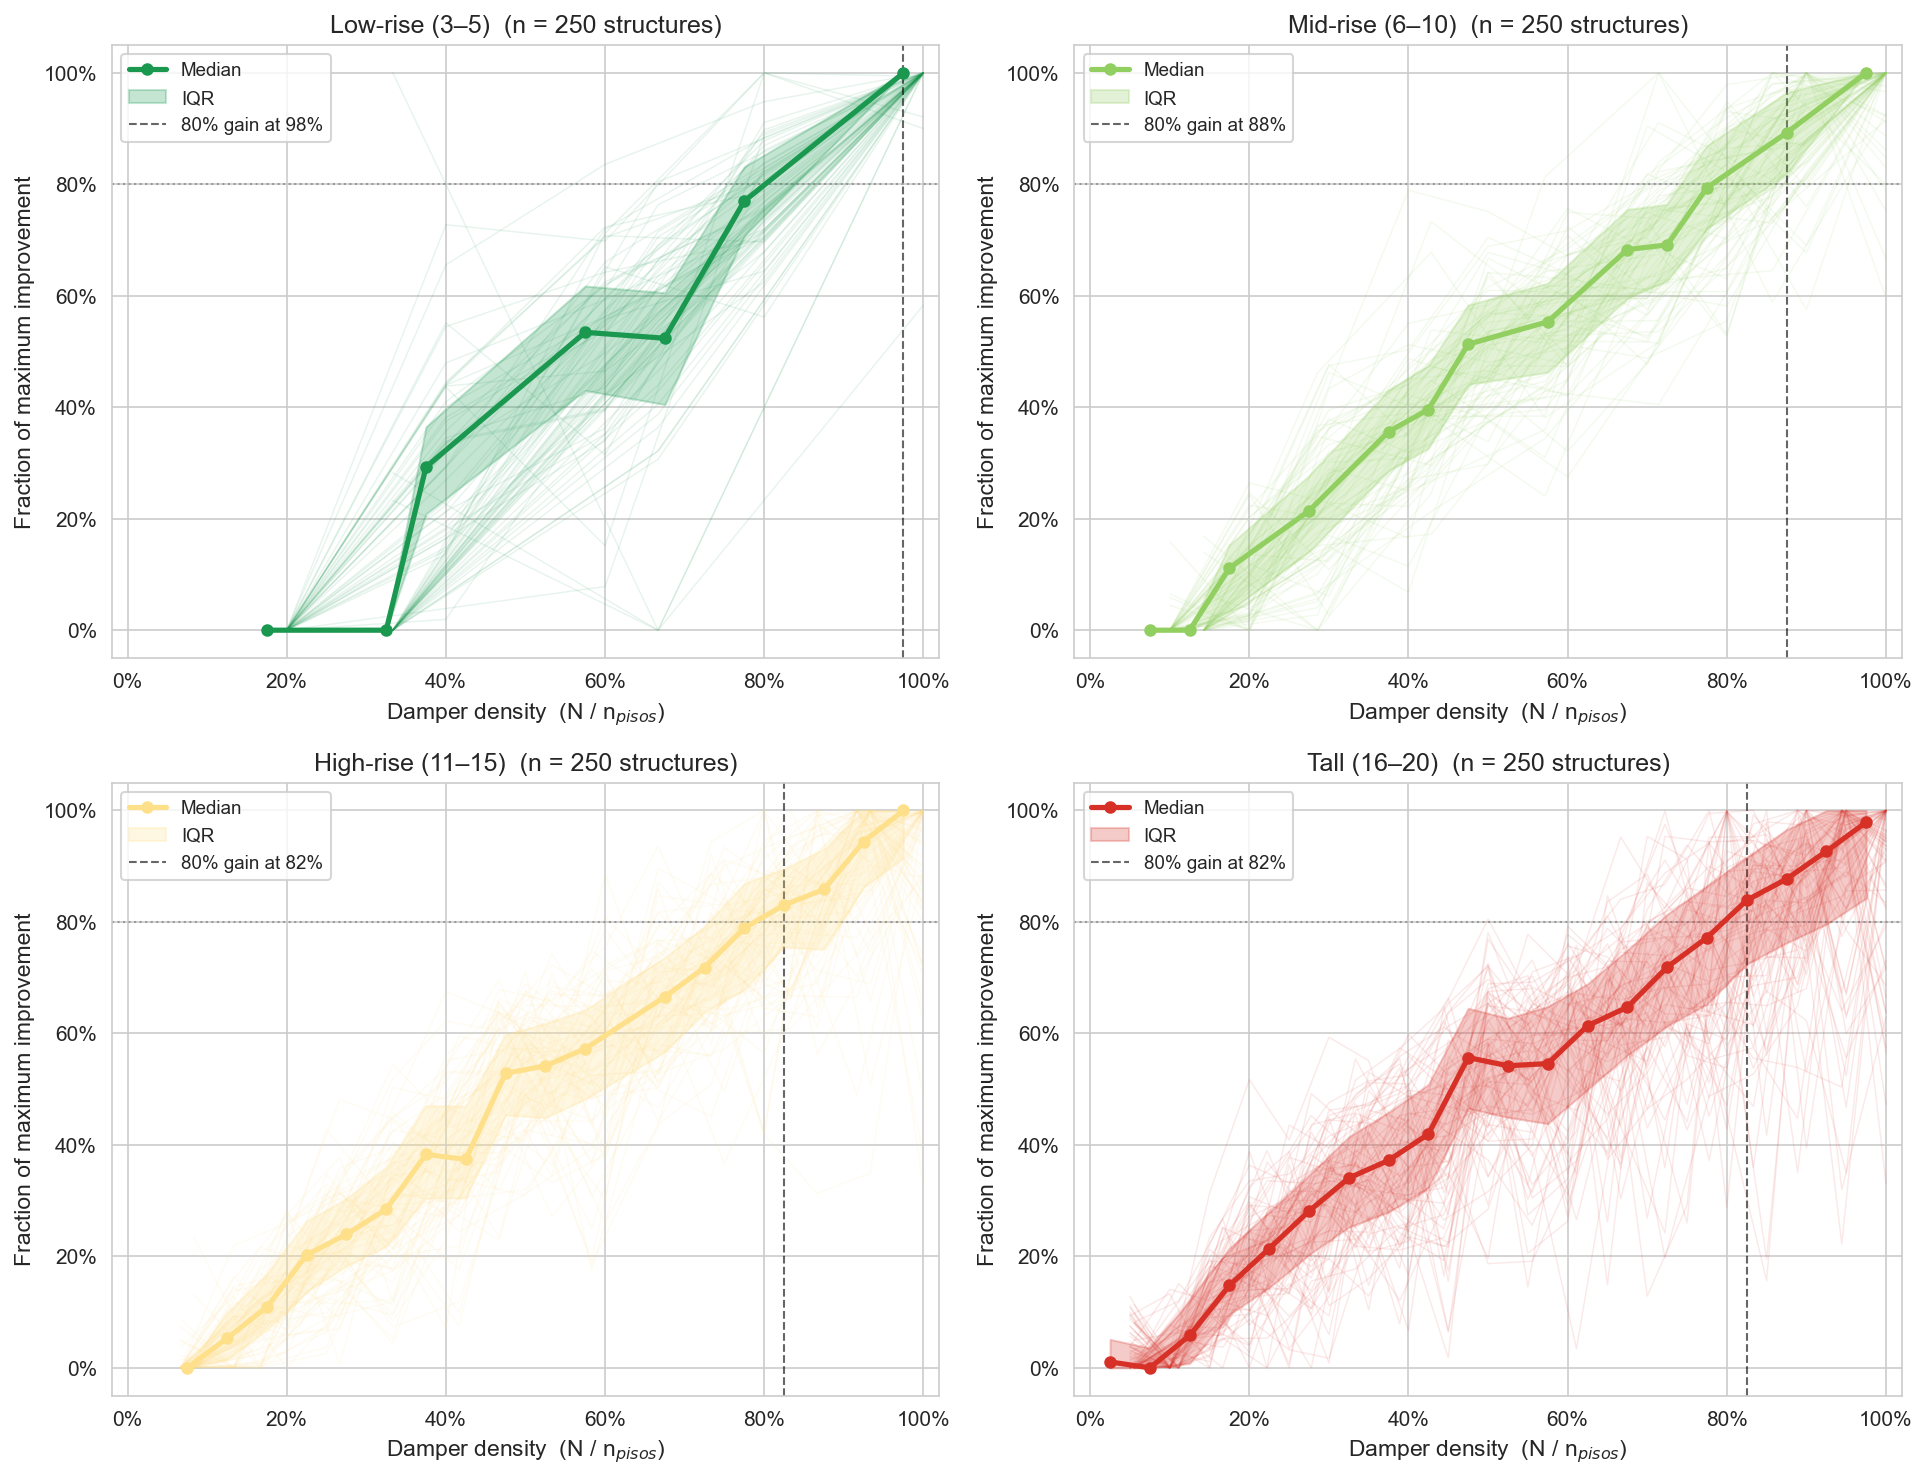
\includegraphics[width=\linewidth]{figs/F6_within_structure_curves.png}
\caption{Within-structure diminishing returns curves by height group. Each thin line represents an
individual structure; thick line is group median $\pm$ IQR. Vertical dashed line: density at which
80\% of maximum gain is achieved.}
\label{fig:curvas_internas}
\end{figure}

\subsection{Interaction between Damper Quantity and Frictional Moment}
\label{sec:results:interaccion}

Figure~\ref{fig:mapa_calor} shows a two-dimensional heatmap of median $CR_2$ as a
function of binned $\nd$ and binned $\Mf$, stratified by three height groups. Stratified
analysis reveals patterns that the global map does not capture.

In all three groups, low density combined with $\Mf \leq 100$\KM produces the highest
$CR_2$ (worst performance), confirming that both variables act as necessary minimum
constraints. The relative weight of each variable changes with building height. In
low-rise frames (3--5 stories), both $\nd$ and $\Mf$ contribute comparably: increasing
$\nd$ from 1--2 to 3--4 with $\Mf \in [200,\,300]$\KM reduces $CR_2$ from 1.46 to
1.12, and raising $\Mf$ from 100 to 300\KM at fixed $\nd$ yields similar reductions,
indicating effective substitution between quantity and capacity. In mid-rise and high-rise
frames (6--20 stories), $\nd$ dominates more clearly: increasing $\Mf$ at any $\nd$
level still improves performance ($\Delta CR_2 \approx 0.37$--$0.46$ across the full
$\Mf$ range), but adding devices consistently outweighs increasing per-device capacity.
Even at high coverage ($\nd \geq 11$), the gap between $\Mf < 100$\KM and
$\Mf > 400$\KM is 0.46 $CR_2$ units for mid-rise frames and 0.37 for tall frames,
showing that $\Mf$ is never irrelevant.

The optimal configurations identified by the ML model across the 1,000 structures
concentrate in $\Mf \in [300,\,460]$\KM (median 400\KM, IQR~[269,\,456]\KM) with
coverage fractions predominantly at or near unity ($\tilde{\eta}_{0.50} = 1.0$).

\begin{figure}[htbp]
\centering
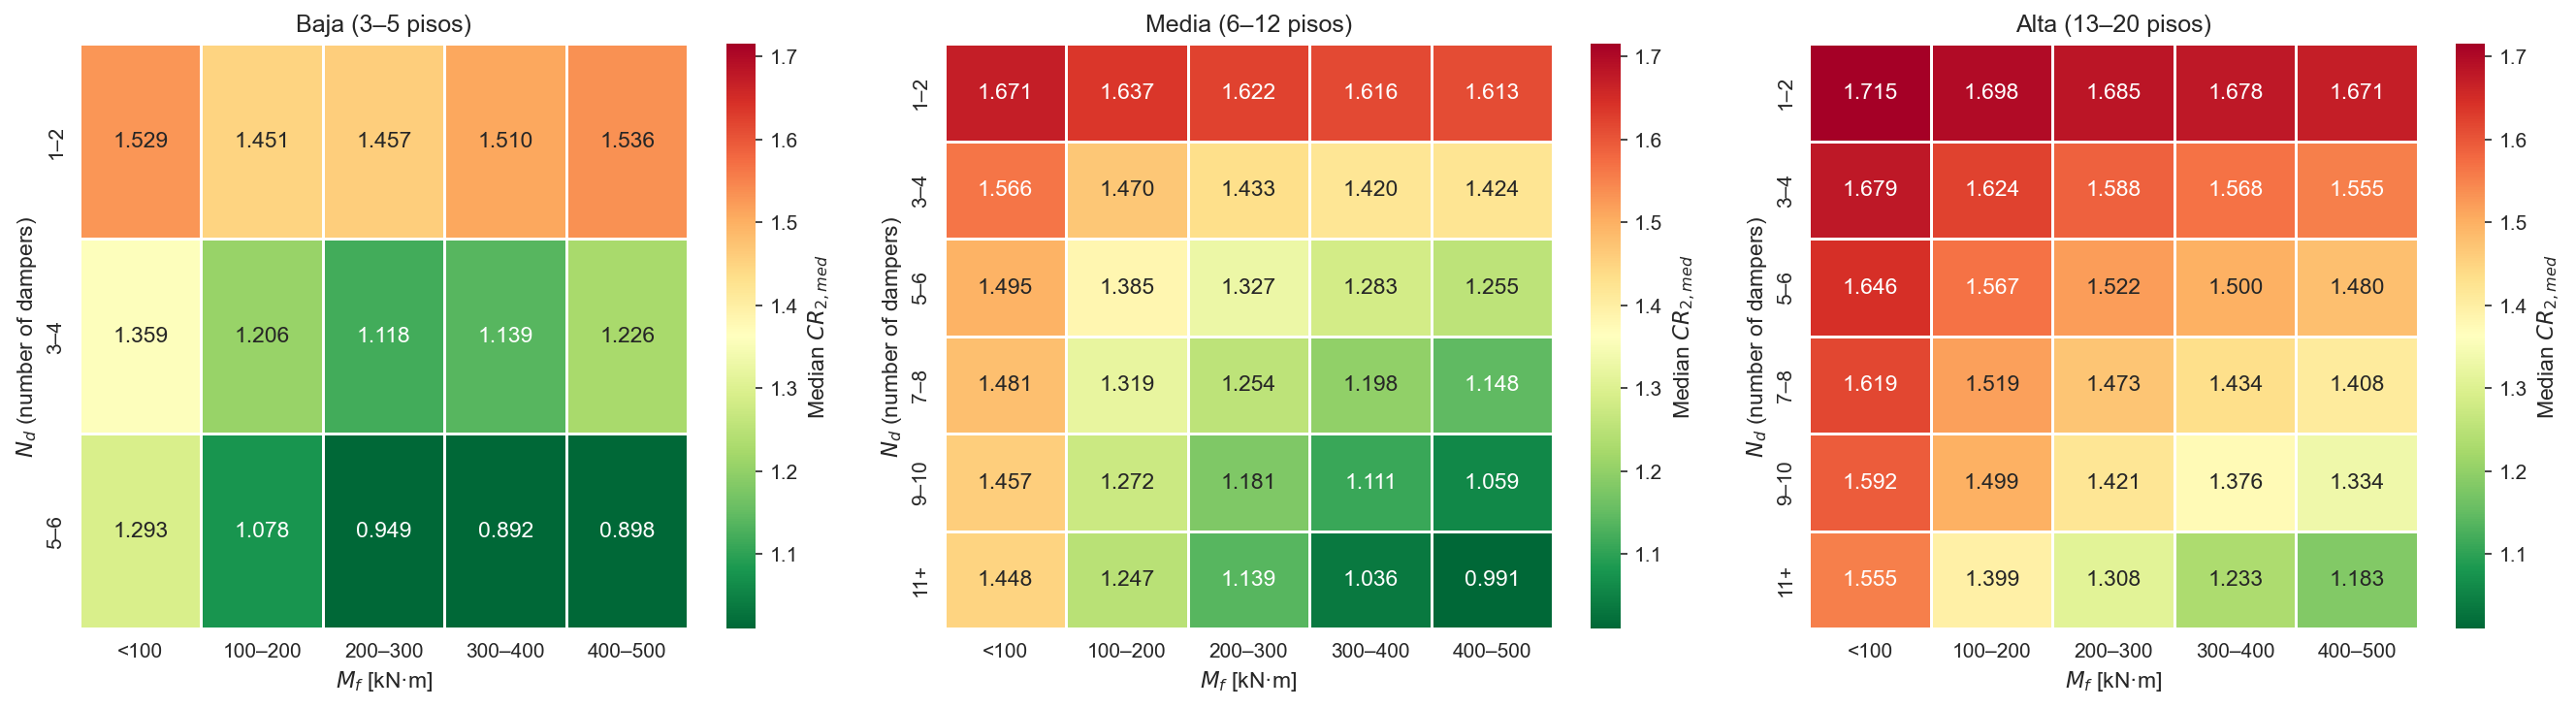
\includegraphics[width=\linewidth]{figs/F7_interaction_heatmap.png}
\caption{Left: median $CR_2$ as a function of $\nd$ bins and $\Mf$ bins (kN$\cdot$m), averaged
across all structures and records. Right: optimal $\nd$ vs.\ $\Mf$ for best configuration of each
structure (color: achieved $\CR{med}$).}
\label{fig:mapa_calor}
\end{figure}

\subsection{Design Convergence across Seismic Scenarios}
\label{sec:results:convergencia}

Figure~\ref{fig:convergencia} examines whether a single optimal RFD design is robust
across the three seismic scenarios. For each of the 1,000 structures, the optimal $\nd$
predicted under each target variable was compared. The distribution of recommended $\nd$
is consistent across scenarios: median and P10 produce nearly identical recommendations
in most structures. The P90 scenario tends to recommend slightly higher $\nd$ for taller
buildings, but the absolute discrepancy
$|\nd^{\mathrm{P90}} - \nd^{\mathrm{med}}|$ stays below 2 for over 80\% of structures.
This means a design optimized for the median scenario provides near-optimal protection
across all seismic variability captured by the eight-record ensemble.

\begin{figure}[htbp]
\centering
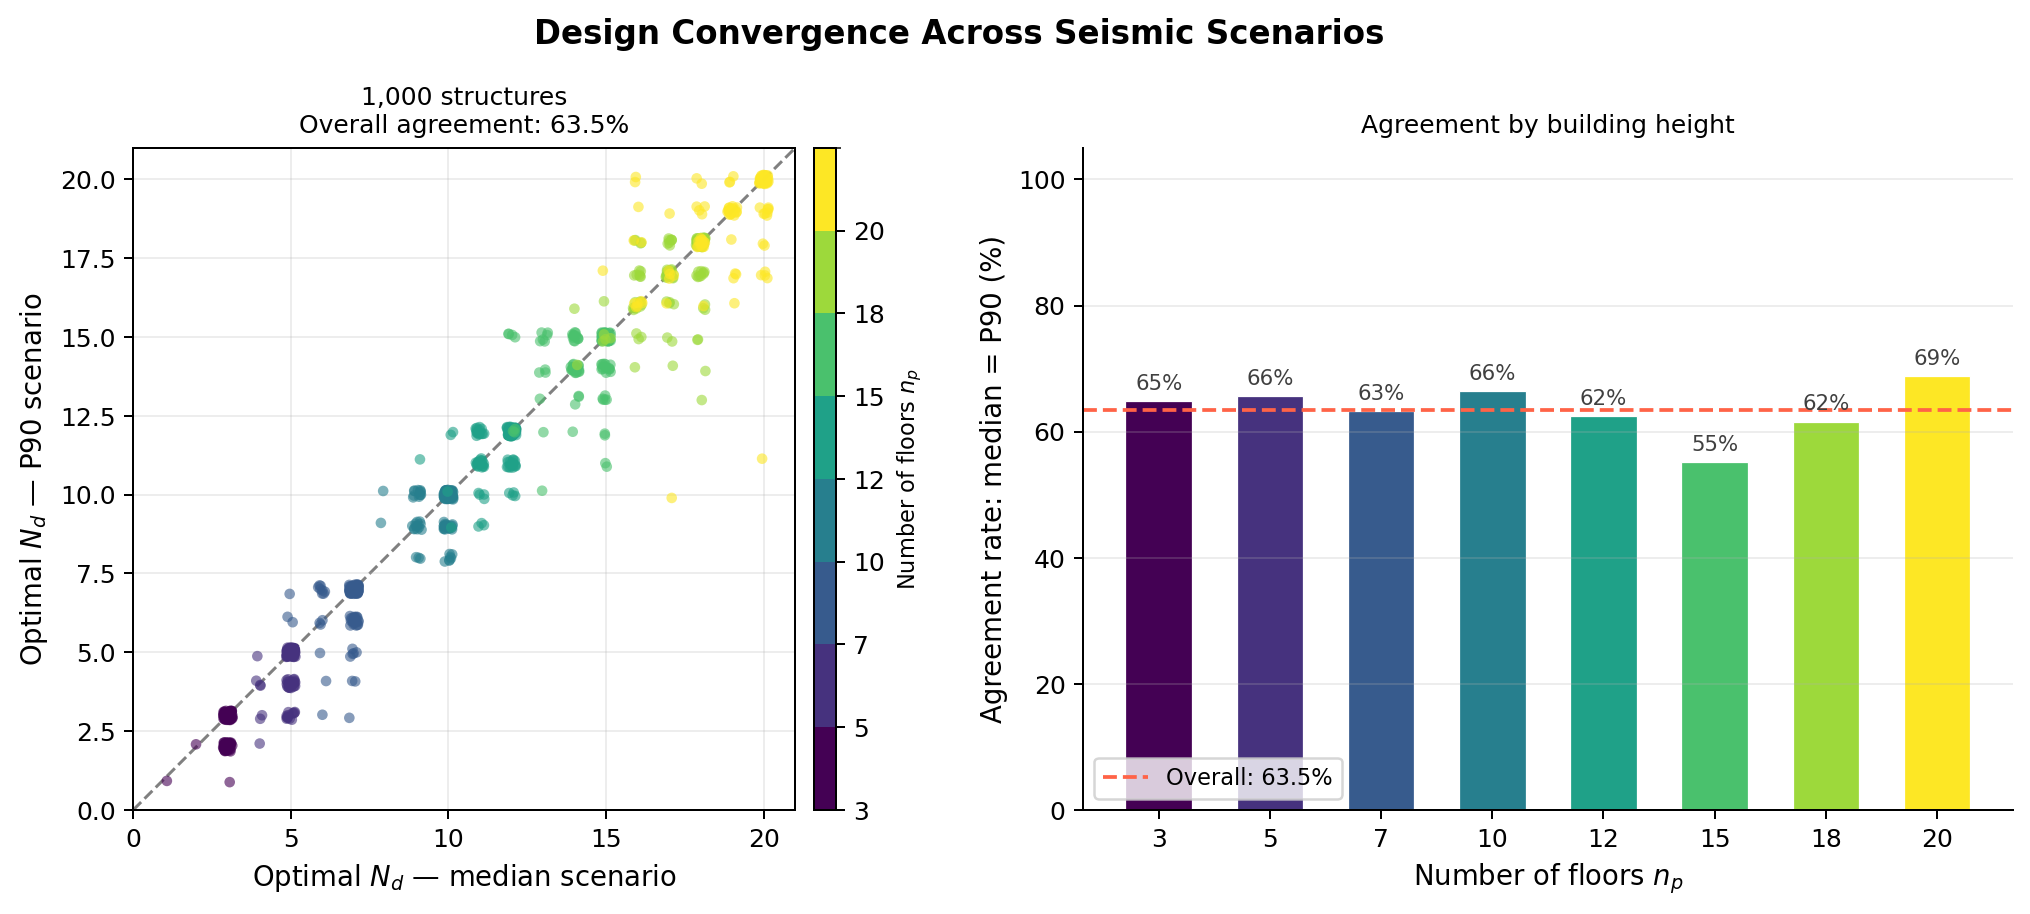
\includegraphics[width=\linewidth]{figs/F8_convergence_extended.png}
\caption{Left: distribution of recommended $\nd$ by seismic scenario across the 1,000 structures.
Right: agreement rate and mean absolute discrepancy $|\nd^{\mathrm{P90}} - \nd^{\mathrm{med}}|$
by building height $\np$.}
\label{fig:convergencia}
\end{figure}

%%═══════════════════════════════════════════════════════════════════════════
\section{Discussion}
\label{sec:discussion}
%%═══════════════════════════════════════════════════════════════════════════

\subsection{Density as Governing Design Parameter}

Coverage density $\etad$ is the dominant predictor of $CR_2$ ($r = -0.73$). Stochastic
dominance analysis confirms that this hierarchy holds across all eight seismic records,
independent of other design variables (Section~\ref{sec:results:decreciente}). From the
80\% maximum gain threshold analysis, the following design recommendation follows:
$\etad \geq 0.85$ for mid-rise and tall frames (6--20 stories), and $\etad \geq 0.90$
for low-rise frames (3--5 stories), where each additional device has proportionally
greater impact.

\subsection{Interaction between Frictional Moment and Coverage}

The heatmap analysis (Figure~\ref{fig:mapa_calor}) reveals a substitution relationship
between $\nd$ and $\Mf$ at intermediate coverage: doubling $\Mf$ at a fixed device
count produces $CR_2$ reductions similar to adding two stories of coverage. This
interaction is not captured by marginal correlation and motivates the use of ensemble ML
models that represent nonlinear feature interactions explicitly. At high coverage
($\etad \geq 0.75$), performance becomes relatively insensitive to the specific $\Mf$
value within [200,\,500]\KM. The ML-identified optimal range, $\Mf \in [300,\,460]$\KM,
is consistent with the optimal $\Mf = 257.9$\,kips$\cdot$in $\approx 290$\KM reported
by \citet{Jarrahi2020jbe} for a single-story MRSF under higher-intensity excitation.

\subsection{Robustness across Scenarios}

The strong agreement between median and P90 design recommendations
(Figure~\ref{fig:convergencia}) means separate optimization problems do not need to be
solved for different hazard levels when the goal is to identify the optimal $\nd$. The
multi-record approach directly addresses the limitation of single-record studies
\citep{Jarrahi2020jbe,Jarrahi2020sdee}, capturing record-to-record variability through
P10, median, and P90 statistics. ML recommendations are therefore inherently robust to
uncertainty in accelerogram selection.

\subsection{Limitations}

The following limitations should be acknowledged. (i)~Structural models are idealized
elastic shear frames; explicit frame--RFD nonlinear interaction is not captured.
(ii)~The eight accelerograms, though seismically diverse, may not represent all relevant
tectonic settings. (iii)~Validation relies only on cross-validation; an independent test
set would provide a more rigorous generalization assessment. (iv)~A uniform $\Mf$ per
structure is assumed; story-specific $\Mf$ distributions may be preferable in practice.
(v)~No cost function is included, so economic optimization of coverage fraction is not
addressed.

%%═══════════════════════════════════════════════════════════════════════════
\section{Conclusions}
\label{sec:conclusions}
%%═══════════════════════════════════════════════════════════════════════════

The following conclusions are drawn from analysis of $\approx$434,000 nonlinear
time-history simulations across 1,000 diverse structural configurations and eight real
seismic records:

\begin{enumerate}

\item \textbf{Accuracy of ML surrogate model.}
XGBoost and Random Forest achieved $\Rsq$ of 0.92--0.93 for $\CR{med}$ and $\CR{P10}$,
and 0.84 for $\CR{P90}$. Ensemble models reduced prediction error by approximately 49\%
relative to linear baselines, quantifying the nonlinear structure of the
design--performance relationship.

\item \textbf{Damper density is the primary design variable.}
Coverage fraction $\etad = \nd/\np$ is the most influential predictor ($r = -0.73$),
substantially outperforming absolute damper count ($r = -0.45$). Design guidelines for
RFDs should be expressed in terms of $\etad$, not $\nd$.

\item \textbf{Diminishing returns threshold: $\etad \approx 0.85$.}
Within-structure analysis shows that 80\% of maximum $CR_2$ reduction is reached at
$\etad \approx 0.85$ for mid-rise and tall frames (6--20~stories) and at
$\etad \approx 0.95$ for low-rise frames (3--5~stories). These thresholds provide
practical cost-effectiveness criteria for RFD deployment.

\item \textbf{Optimal range of frictional moment.}
Across the 1,000 structures, ML identifies optimal $\Mf$ in [300,\,460]\KM (median
400\KM). For $\etad \geq 0.75$, $CR_2$ is relatively insensitive to the specific $\Mf$
value within [200,\,500]\KM, making coverage fraction the most critical design parameter.

\item \textbf{Robustness across scenarios.}
Optimal $\nd$ recommended by median and P90 scenarios differs by fewer than 2 stories in
80\% of analyzed structures. A design optimized for the median scenario provides
near-optimal protection across all seismic variability in the eight-record ensemble.

\item \textbf{Future work.}
Extensions should incorporate inelastic frame behavior, story-specific $\Mf$
distributions, installation cost constraints, and broader seismic record suites covering
different tectonic environments. Experimental validation for multi-story configurations
and integration of trained models into an interactive design tool are immediate research
directions.

\end{enumerate}

%%═══════════════════════════════════════════════════════════════════════════
\bibliographystyle{elsarticle-harv}
\bibliography{references}

\end{document}
